\documentclass[12pt, twoside]{article} % Definuje typ dokumentu (článek)
\usepackage[
    inner=3cm,      % Okraj u hřbetu (vnitřní)
    outer=2.2cm,    % Vnější okraj
    top=2.5cm,      % (Doporučeno definovat i nahoře/dole)
    bottom=2.5cm
]{geometry}

\usepackage[utf8]{inputenc}
\usepackage{graphicx}
\usepackage{tikz}
\usepackage{circuitikz}
\usetikzlibrary{shapes.geometric, arrows.meta}

\tikzset{
    startstop/.style = {rectangle, rounded corners, minimum width=2.8cm, minimum height=1cm, text centered, draw=black, fill=red!30, text width=2.7cm},
    process/.style = {rectangle, minimum width=2.8cm, minimum height=1cm, text centered, draw=black, fill=orange!30, text width=2.7cm},
    decision/.style = {diamond, minimum width=2.8cm, minimum height=1cm, text centered, draw=black, fill=yellow!30, text width=2cm, inner sep=0pt},
    arrow/.style = {thick, ->, >=stealth}
}
\usepackage{mathptmx}
\usepackage{setspace}
\onehalfspacing
\usepackage{microtype}
\usepackage{float}
\usepackage{listings}
\usepackage{xcolor} % Pro barvy

\usepackage[backend=biber, style=numeric]{biblatex}
\addbibresource{literatura.bib}

\lstset{
    language=C++,
    basicstyle=\ttfamily\small, % Písmo stroje
    keywordstyle=\color{blue}\bfseries,
    stringstyle=\color{red},
    commentstyle=\color{green!50!black},
    numbers=left, % Číslování řádků
    numberstyle=\tiny\color{gray},
    frame=single, % Rámeček okolo
    breaklines=true % Zalamování dlouhých řádků
}

\newcommand{\Univerzita}{Jihočeská univerzita v Českých Budějovicích}
\newcommand{\Fakulta}{Přírodovědecká fakulta}
\newcommand{\NazevPrace}{Hlídací systém kotelny s využítím platformy Blynk}
\newcommand{\TypPrace}{Semestrální práce}
\newcommand{\Autor}{Vít Horčička}

\newcommand{\MestoRok}{České Budějovice 2026}

\begin{document} % Začátek obsahu

\begin{titlepage}
    \centering
    
    % --- HLAVIČKA ---
    {\fontsize{14pt}{17pt}\selectfont \bfseries
    \Univerzita \\       % Použití proměnné
    \Fakulta \par}       % Použití proměnné
    
    \vspace{4cm}
    
    % --- NÁZEV PRÁCE ---
    {\fontsize{18pt}{22pt}\selectfont \bfseries
    \NazevPrace \par}
    
    \vspace{2cm}
    
    % --- TYP PRÁCE ---
    {\fontsize{18pt}{22pt}\selectfont \bfseries
    \TypPrace \par}
    
    \vspace{1.5cm}
    
    % --- AUTOR ---
    
    \vfill 
        {\Large \textbf{\Autor} \par}

    
    \vspace{1cm}
    
    % --- MÍSTO A ROK ---
    {\large \MestoRok \par}
\end{titlepage}

\newpage
\tableofcontents
\newpage

\section*{Seznam zkratek}
\addcontentsline{toc}{section}{Seznam zkratek} % Add to table of contents
\begin{itemize}
    \item IoT - Internet of Things (Internet věcí)
    \item ESP32 - Expressif Systems 32 (Mikrokontrolér)
    \item I2C - Inter-Integrated Circuit (Komunikační protokol)
    \item MQTT - Message Queuing Telemetry Transport (Komunikační protokol)
    \item LED - Light Emitting Diode (Světlo emitující dioda)
    \item GND - Ground (Zem)
    \item 3V3 - 3.3 Volts (Napájecí napětí)
    \item VCC, VIN - Voltage Common Collector (Napájecí napětí)
    \item Wi-Fi - Wireless Fidelity (Bezdrátová technologie)
    \item API - Application Programming Interface (Rozhraní pro programování aplikací)
\end{itemize}
\newpage

\section{Úvod}
Tato semestrální práce se zabývá návrhem a implementací hlídacího systému pro kotelnu s využitím platformy Blynk. V kontextu moderních chytrých domácností je automatizované monitorování a řízení klíčových systémů, jako je vytápění, nejen otázkou komfortu, ale především bezpečnosti a efektivity. Cílem této práce je vytvořit cenově dostupný a spolehlivý systém, který bude v reálném čase sledovat kritické parametry v kotelně – konkrétně teplotu, vlhkost, tlak a přítomnost nebezpečných plynů.

Práce je strukturována následovně: nejprve je představen koncept chytré domácnosti a problematika spojená s monitorováním kritických systémů. Následně je popsán hardware, včetně mikrokontroleru ESP32 a senzorů BME280 a MQ135, a softwarové řešení postavené na platformě Blynk. Další kapitoly se věnují detailnímu návrhu zapojení, signalizačním mechanismům a softwarové logice. V závěru jsou shrnuty dosažené výsledky, diskutovány nalezené problémy a navrženy možnosti dalšího rozšíření.

Výsledný systém umožní uživateli vzdáleně sledovat stav kotelny prostřednictvím mobilní aplikace, přijímat okamžitá varování v případě anomálií a mít tak neustálý přehled o bezpečnosti a funkčnosti vytápěcího systému.

\subsection{Internet věcí (IoT)}
Internet věcí (IoT) představuje rozsáhlou síť fyzických zařízení, vozidel, domácích spotřebičů a dalších předmětů, které jsou vybaveny senzory, softwarem a dalšími technologiemi umožňujícími připojení a výměnu dat s jinými zařízeními a systémy přes internet. Tato konektivita umožňuje vzdálený monitoring, sběr dat, analýzu a automatizaci procesů v reálném čase. Cílem IoT je zvýšit efektivitu, přesnost a ekonomický přínos v široké škále aplikací, od průmyslových systémů přes chytrá města až po osobní zařízení a domácnosti. V kontextu monitorovacích systémů, jako je ten v této práci, IoT poskytuje základní infrastrukturu pro sběr dat z fyzického světa a jejich zpřístupnění pro analýzu a akci. \autocite{wiki:iot}

\subsection{Chytrá domácnost}
Chytrá domácnost, známá také jako inteligentní dům, je koncept bydlení, který zajišťuje optimální vnitřní prostředí pro život obyvatel. Toho je dosaženo souhrou stavební konstrukce, technologií, automatizovaného řízení a služeb. Cílem je zvýšit komfort, zlepšit zábavu, zajistit bezpečnost a snížit provozní náklady. Systém je obvykle modulární a jeho centrální jednotka automatizuje operace jako vytápění, osvětlení, zabezpečení a zábavu, přičemž vše je ovladatelné prostřednictvím různých rozhraní \autocite{wiki:inteligentni_dum}.

\subsection{Problematika spolehlivosti a řízení rizik}
Při návrhu jakéhokoliv technického systému, jehož selhání může způsobit materiální škody nebo ohrozit zdraví, je nutné zohlednit principy řízení rizik. Cílem je identifikovat potenciální hrozby, analyzovat jejich pravděpodobnost a dopad a navrhnout opatření k jejich minimalizaci. Klíčovými pojmy jsou zde \textbf{spolehlivost} (schopnost systému plnit požadovanou funkci po danou dobu), \textbf{bezpečnost} (schopnost systému nezpůsobit nepřijatelné riziko) a \textbf{dostupnost} (pravděpodobnost, že systém bude v daném čase funkční). Ačkoliv monitorovací systém kotelny není formálně klasifikován jako kritický, aplikujeme tyto principy pro zajištění jeho robustnosti.

\subsubsection{Specifika IoT a závislost na cloudu}
U systémů spadajících do kategorie Internetu věcí (IoT) vstupuje do hry specifický rizikový faktor: závislost na externích službách a konektivitě. Využití cloudové platformy, jako je Blynk, přináší řadu výhod, ale také významná rizika, která je třeba řídit.

\paragraph*{Výhody cloudového řešení}
\begin{itemize}
    \item \textbf{Vzdálený přístup:} Uživatel může kdykoliv a odkudkoliv kontrolovat stav kotelny prostřednictvím mobilní aplikace.
    \item \textbf{Okamžité notifikace:} V případě detekce anomálie (např. únik plynu) systém okamžitě odešle varování na mobilní zařízení uživatele, což umožňuje rychlou reakci.
    \item \textbf{Vizualizace a historie dat:} Cloudová platforma umožňuje přehledné zobrazení aktuálních i historických dat v grafech, což usnadňuje sledování trendů a diagnostiku problémů.
    \item \textbf{Jednoduchost implementace:} Hotová platforma výrazně zjednodušuje vývoj, protože není nutné programovat vlastní serverovou a mobilní aplikaci.
\end{itemize}

\paragraph*{Nevýhody a rizika}
\begin{itemize}
    \item \textbf{Závislost na připojení k internetu:} Celá vzdálená funkčnost je závislá na stabilním internetovém připojení jak v místě instalace, tak na straně uživatele. Při výpadku se ztrácí možnost monitorování a přijímání notifikací.
    \item \textbf{Závislost na třetí straně:} Systém je závislý na dostupnosti a podpoře služby Blynk. Pokud má poskytovatel technický výpadek nebo službu v budoucnu ukončí, systém ztratí svou klíčovou funkcionalitu.
    \item \textbf{Potřeba lokální autonomie:} Z výše uvedených důvodů je nezbytné, aby zařízení mělo základní autonomní funkce. V této práci je to řešeno lokální optickou signalizací (LED diody), která varuje osoby v bezprostřední blízkosti zařízení i bez funkčního připojení k cloudu.
    \item \textbf{Bezpečnostní rizika:} Připojení k internetu otevírá systém potenciálním kybernetickým útokům. Je nutné dbát na silné zabezpečení sítě a přístupových údajů k platformě.
\end{itemize}

\newpage

\section{Systém monitorování kotelny}
Pro monitorování prostředí v kotelně budou použity následující principy a technologie:
\subsection{Laskakit ESP32}
ESP32 je výkonný mikrokontrolér s integrovanou Wi-Fi a Bluetooth konektivitou, který je ideální pro IoT projekty. Jeho schopnost připojení k internetu umožňuje odesílání dat do cloudových služeb, jako je Blynk, a umožňuje vzdálené ovládání zařízení. ESP32 bude sloužit jako centrální jednotka pro sběr dat ze senzorů a komunikaci s platformou Blynk. \autocite{laskakit_esp32}
\subsection{Komunikace}
Pro komunikaci mezi senzory a ESP32 bude využit protokol I2C, který umožňuje připojení více zařízení na stejné sběrnici. Data ze senzorů budou pravidelně odesílána do platformy Blynk, kde budou zpracovávána a vizualizována pro uživatele.
Pro komunikaci s platformou Blynk bude využit protokol MQTT, který je optimalizován pro nízkou latenci a nízkou spotřebu energie, což je ideální pro IoT zařízení. ESP32 bude fungovat jako MQTT klient, který bude odesílat data do Blynk serveru a přijímat příkazy od uživatele. \autocite{blynk_docs}
\subsection{Senzory}
\subsubsection{BME280}
Senzor BME280 je integrovaný senzor od společnosti Bosch Sensortec, který dokáže měřit atmosférický tlak, relativní vlhkost a teplotu. Vyznačuje se vysokou přesností a nízkou spotřebou energie, což jej činí ideálním pro monitorovací aplikace. Data ze senzoru BME280 jsou klíčová pro sledování podmínek v kotelně a identifikaci potenciálních abnormalit.
\subsubsection{MQ135}
Senzor MQ135 je senzor kvality ovzduší, který je schopen detekovat širokou škálu plynů, včetně amoniaku, sirovodíku, benzenu, alkoholu, kouře a oxidu uhličitého. Jeho citlivost na tyto plyny umožňuje monitorovat znečištění vzduchu a přítomnost nebezpečkých látek v prostředí kotelny. Signál z MQ135 je důležitý pro posouzení celkové kvality ovzduší a včasné varování před rizikovými koncentracemi plynů. \autocite{dratek_mq135}

\subsection{Komponenty}
\subsubsection{Nepájivé pole (Breadboard)}
Pro snadné a rychlé prototypování bez nutnosti pájení je použit breadboard. Umožňuje flexibilní propojování jednotlivých komponent, jako jsou senzory a LED diody, s mikrokontrolérem ESP32.

\subsubsection{LED diody}
V projektu jsou použity tři LED diody různých barev (zelená, žlutá, červená) pro vizuální signalizaci stavu systému. Jejich specifické funkce pro indikaci normálního provozu, varování a kritických stavů jsou popsány v kapitole \ref{sec:signalizace_led}.

\section{Návrh zapojení a signalizace}
Pro realizaci monitorovacího systému kotelny bude použito následující zapojení:
\begin{figure}[H]
    \centering
    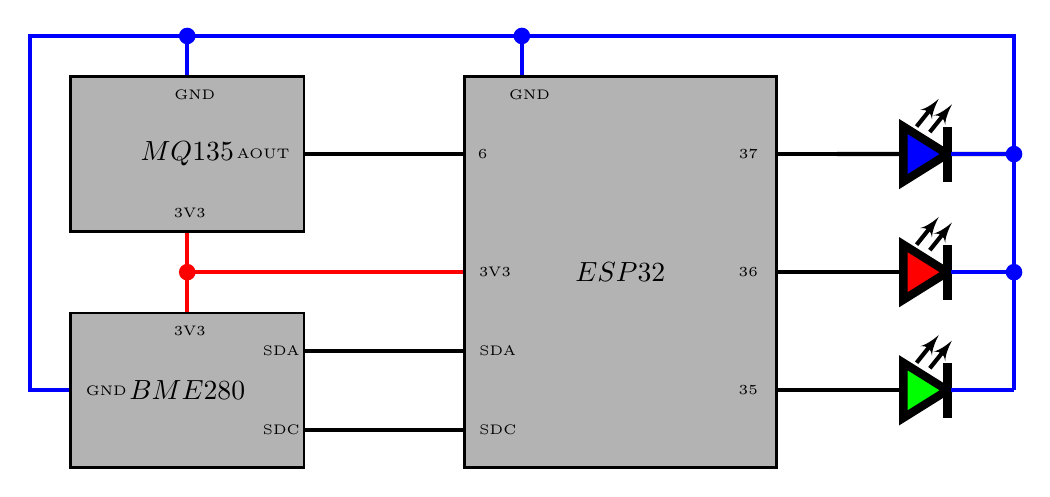
\begin{tikzpicture}
	\draw[line width=1.5pt] (14.75, 11) to[led, fill=blue] (17, 11);
	\draw[line width=1.5pt, blue] (16.2, 11) -- (17, 11);
	
	\draw[line width=1.5pt] (14.75, 9.5) to[led, fill=red] (17, 9.5);
	\draw[line width=1.5pt, blue] (16.2, 9.5) -- (17, 9.5);
	
	\draw[line width=1.5pt] (14.75, 8) to[led, fill=green] (17, 8);
	\draw[line width=1.5pt, blue] (16.2, 8) -- (17, 8);

	\node[shape=rectangle, fill={rgb,255:red,179;green,179;blue,179}, draw, line width=1pt, minimum width=3.965cm, minimum height=4.965cm](N1) at (12, 9.5){} node[anchor=center] at (N1.text){$ESP 32 $};
	\node[shape=rectangle, fill={rgb,255:red,179;green,179;blue,179}, draw, line width=1pt, minimum width=2.965cm, minimum height=1.965cm](N2) at (6.5, 11){} node[anchor=center] at (N2.text){$MQ135$};
	\node[shape=rectangle, fill={rgb,255:red,179;green,179;blue,179}, draw, line width=1pt, minimum width=2.965cm, minimum height=1.965cm](N3) at (6.5, 8){} node[anchor=center] at (N3.text){$BME 280$};

	\draw[line width=1.5pt, blue] (10.75, 12) -| (10.75, 12.5);
	\draw[line width=1.5pt, blue] (10.75, 12.5) -- (6.5, 12.5) -| (6.5, 12);
	\draw[line width=1.5pt, blue] (10.75, 12.5) -- (17, 12.5) -| (17, 8);
	\draw[line width=1.5pt, blue] (5, 8) -- (4.5, 8) -- (4.5, 12.5) -- (6.5, 12.5);
	
	\draw[line width=1.5pt] (14.75, 11) -- (14, 11);
	\draw[line width=1.5pt] (14.75, 9.5) -- (14, 9.5);
	\draw[line width=1.5pt] (14.75, 8) -- (14, 8);
	\draw[line width=1.5pt] (8, 11) -- (10, 11);
	\draw[line width=1.5pt] (8, 8.5) -- (10, 8.5);
	\draw[line width=1.5pt] (10, 7.5) -- (8, 7.5);
	
	\draw[line width=1.5pt, red] (6.5, 9) -- (6.5, 10);
	\draw[line width=1.5pt, red] (6.5, 9.5) -- (10, 9.5);

	\fill[blue] (10.75, 12.5) circle (3pt);
	\fill[blue] (6.5, 12.5) circle (3pt);
	\fill[blue] (17, 11) circle (3pt);
	\fill[blue] (17, 9.5) circle (3pt);
	\fill[red] (6.5, 9.5) circle (3pt);
	
	\node[shape=rectangle, minimum width=0.715cm, minimum height=0.465cm] at (10.75, 11.75){} node[anchor=center, align=center, text width=0.327cm, inner sep=6pt] at (10.75, 11.75){\tiny GND};
	\node[shape=rectangle, minimum width=0.715cm, minimum height=0.465cm] at (6.5, 11.75){} node[anchor=center, align=center, text width=0.327cm, inner sep=6pt] at (6.5, 11.75){\tiny GND};
	\node[shape=rectangle, minimum width=0.715cm, minimum height=0.465cm] at (5.375, 8){} node[anchor=center, align=center, text width=0.327cm, inner sep=6pt] at (5.375, 8){\tiny GND};
	\node[shape=rectangle, minimum width=0.715cm, minimum height=0.465cm] at (10.375, 9.5){} node[anchor=center, align=center, text width=0.327cm, inner sep=6pt] at (10.375, 9.5){\tiny 3V3};
	\node[shape=rectangle, minimum width=0.715cm, minimum height=0.465cm] at (6.5, 8.75){} node[anchor=center, align=center, text width=0.327cm, inner sep=6pt] at (6.5, 8.75){\tiny 3V3};
	\node[shape=rectangle, minimum width=0.715cm, minimum height=0.465cm] at (6.5, 10.25){} node[anchor=center, align=center, text width=0.327cm, inner sep=6pt] at (6.5, 10.25){\tiny 3V3};
	\node[shape=rectangle, minimum width=0.715cm, minimum height=0.465cm] at (10.25, 11){} node[anchor=center, align=center, text width=0.327cm, inner sep=6pt] at (10.25, 11){\tiny 6};
	\node[shape=rectangle, minimum width=0.715cm, minimum height=0.465cm] at (7.3, 11){} node[anchor=center, align=center, text width=0.327cm, inner sep=6pt] at (7.3, 11){\tiny AOUT};
	\node[shape=rectangle, minimum width=0.715cm, minimum height=0.465cm] at (7.625, 8.5){} node[anchor=center, align=center, text width=0.327cm, inner sep=6pt] at (7.625, 8.5){\tiny SDA};
	\node[shape=rectangle, minimum width=0.715cm, minimum height=0.465cm] at (13.625, 8){} node[anchor=center, align=center, text width=0.327cm, inner sep=6pt] at (13.625, 8){\tiny 35};
	\node[shape=rectangle, minimum width=0.715cm, minimum height=0.465cm] at (10.375, 8.5){} node[anchor=center, align=center, text width=0.327cm, inner sep=6pt] at (10.375, 8.5){\tiny SDA};
	\node[shape=rectangle, minimum width=0.715cm, minimum height=0.465cm] at (7.625, 7.5){} node[anchor=center, align=center, text width=0.327cm, inner sep=6pt] at (7.625, 7.5){\tiny SDC};
	\node[shape=rectangle, minimum width=0.715cm, minimum height=0.465cm] at (10.375, 7.5){} node[anchor=center, align=center, text width=0.327cm, inner sep=6pt] at (10.375, 7.5){\tiny SDC};
	\node[shape=rectangle, minimum width=0.715cm, minimum height=0.465cm] at (13.625, 9.5){} node[anchor=center, align=center, text width=0.327cm, inner sep=6pt] at (13.625, 9.5){\tiny 36};
	\node[shape=rectangle, minimum width=0.715cm, minimum height=0.465cm] at (13.625, 11){} node[anchor=center, align=center, text width=0.327cm, inner sep=6pt] at (13.625, 11){\tiny 37};
\end{tikzpicture}
    \caption{Diagram zapojení monitorovacího systému kotelny. Vytvořeno pomocí \autocite{circuit2tikz_designer}}
    \label{fig:flowchart}
\end{figure}ESP32 bude připojen k senzoru BME280 pomocí I2C rozhraní a k senzoru MQ135 pomocí analogového vstupu. K signalizaci různých stavů systému budou použity LED diody.


\subsection{Signalizace LED diod}
\label{sec:signalizace_led}
Pro indikaci různých stavů systému budou použity LED diody s následujícími funkcemi:
\begin{itemize}
    \item \textbf{Zelená LED:} Indikuje normální provoz a bezpečné podmínky v kotelně.
    \item \textbf{Žlutá LED:} Indikuje mírné odchylky od normálních podmínek, které mohou vyžadovat pozornost, například mírně zvýšenou teplotu nebo vlhkost.
    \item \textbf{Červená LED:} Indikuje kritické podmínky, jako je přehřátí, únik plynu nebo vysoká koncentrace škodlivých látek, které vyžadují okamžitou reakci.
\end{itemize}

\section{Návrh funkčnosti}
Systém bude v pravidelných intervalech sbírat data ze senzorů a kontrolovat je proti předem definovaným prahům. Pokud budou detekovány odchylky, systém bude aktualizovat stav LED diod a odesílat upozornění do platformy Blynk, kde bude uživatel informován o aktuálním stavu kotelny a případných rizicích.
V určitých časových intervalech bude systém také odesílat data do Blynk pro dlouhodobé sledování a analýzu trendů, což umožní uživateli lépe porozumět podmínkám v kotelně a případně optimalizovat její provoz.

\subsection{Diagram programu}
Pro lepší pochopení logiky programu pro monitorovací systém kotelny je níže uveden diagram, který znázorňuje hlavní funkční bloky a jejich vzájemné interakce.
\begin{figure}[H]
    \centering
    
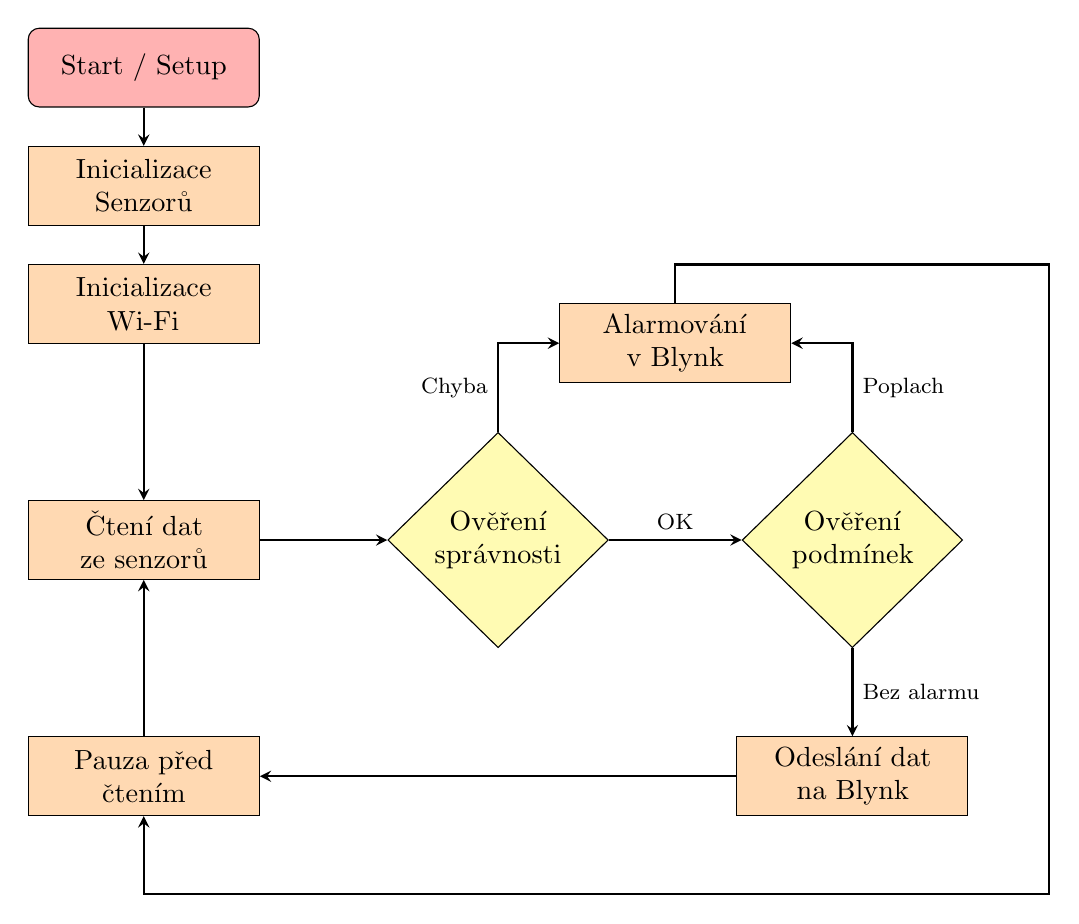
\begin{tikzpicture}
    \node (start) [startstop] at (0, 8) {Start / Setup};
    \node (initsens) [process] at (0, 6.5) {Inicializace Senzorů};
    \node (initwifi) [process] at (0, 5) {Inicializace Wi-Fi};
    
    \node (read) [process] at (0, 2) {Čtení dat ze senzorů};
    \node (verify) [decision] at (4.5, 2) {Ověření správnosti};
    \node (alarm) [decision] at (9, 2) {Ověření podmínek};
    
    \node (blynkalarm) [process] at (6.75, 4.5) {Alarmování v Blynk};
    
    \node (blynk) [process] at (9, -1) {Odeslání dat na Blynk};
    \node (wait) [process] at (0, -1) {Pauza před čtením};

    \draw [arrow] (start) -- (initsens);
    \draw [arrow] (initsens) -- (initwifi);
    \draw [arrow] (initwifi) -- (read);

    \draw [arrow] (read) -- (verify);
    \draw [arrow] (verify) -- node[above] {\footnotesize OK} (alarm);
    
    \draw [arrow] (verify.north) |- node[near start, left] {\footnotesize Chyba} (blynkalarm.west);
    \draw [arrow] (alarm.north) |- node[near start, right] {\footnotesize Poplach} (blynkalarm.east);
    
    \draw [arrow] (alarm.south) -- node[right] {\footnotesize Bez alarmu} (blynk.north);
    
    \draw [arrow] (blynk.west) -- (wait.east);
    \draw [arrow] (wait.north) -- (read.south);
    
    \draw [arrow] (blynkalarm.north) |- (11.5, 5.5) |- (0, -2.5) -- (wait.south);
\end{tikzpicture}

    \caption{Diagram programu pro monitorovací systém kotelny.}
\end{figure}

\subsection{Programový kód}
Programový kód pro ESP32 bude napsán v jazyce C++ a bude využívat knihovny pro komunikaci s Blynk, I2C a analogové vstupy. Kód bude strukturován tak, aby byl snadno čitelný a udržovatelný, s jasně definovanými funkcemi pro sběr dat, kontrolu prahů, aktualizaci LED diod a komunikaci s platformou Blynk. Příklad ukazuje logiku posuzování dat ze senzorů a aktualizace stavu LED diod:
\begin{lstlisting}
#include <Wire.h>
#include <BlynkSimpleEsp32.h>
#include <Adafruit_BME280.h>
\end{lstlisting}


\section{Závěr}
Monitorovací systém kotelny s využitím platformy Blynk představuje efektivní řešení pro sledování a řízení podmínek v kotelně. Díky integraci senzorů BME280 a MQ135, spolu s výkonným mikrokontrolérem ESP32, je systém schopen poskytovat uživatelům důležité informace o stavu kotelny a umožnit jim rychle reagovat na potenciální hrozby. Ačkoliv tento systém není kritickým systémem v pravém slova smyslu, aplikuje některé z principů řízení rizik a bezpečnosti, které jsou klíčové pro zajištění bezpečného a spolehlivého provozu v prostředí kotelny.

\subsection{Nalezené problémy}
Během vývoje systému byly identifikovány následující problémy:
\begin{itemize}
    \item \textbf{Omezená spolehlivost senzoru MQ135:} Tento senzor může být náchylný k falešným pozitivům a negativům, což může vést k nesprávným indikacím stavu vzduchu v kotelně.
    \item \textbf{Závislost na připojení k internetu:} Systém je závislý na stabilním připojení k internetu pro komunikaci s platformou Blynk, což může být problém v případě výpadku sítě.
    \item \textbf{Omezené možnosti rozšíření:} Systém je navržen pro konkrétní sadu senzorů a funkcí, což může omezit jeho schopnost přizpůsobit se budoucím potřebám nebo integraci s dalšími zařízeními v rámci chytré domácnosti.
\end{itemize}

\nocite{*}
\newpage
\printbibliography[heading=bibintoc,title={Seznam použité literatury}]


\end{document} % Konec obsahu